\documentclass{beamer}
%\usetheme{Warsaw}
%\usetheme{Madrid}
\usetheme{Marburg}
\usecolortheme{albatross}
\setbeamercovered{transparent}
\usepackage[english]{babel}

% Title page details
\title{Qubes OS Documentation Localization}
\subtitle{Past, Present, Future}
\author{m, Tobias Killer}
\institute{}
\date{September 10, 2022}

\begin{document}

\begin{frame}
	\titlepage
\end{frame}

%\begin{frame}
%	\frametitle{Frames und Slides}
%	\framesubtitle{Frames}
%	\begin{itemize}
%		\item<1> erster Punkt
%		\item<2> zweiter Punkt
%		\item<3> dritter Punkt
%	\end{itemize}
%	\begin{block}{Ein Standardblock}
%	\end{block}
%	\begin{exampleblock}{Ein Beispielblock}
%	\end{exampleblock}
%	\begin{alertblock}{Ein Alarmblock}
%	\end{alertblock}
%\end{frame}

\AtBeginSection[]
{
\begin{frame}<beamer>
\frametitle{Outline}
\tableofcontents[currentsection]
\end{frame}
}

\begin{frame}
	\frametitle{Outline}
	\tableofcontents
\end{frame}

\section{Introduction \& Welcome (m) )}

\begin{frame}
	\frametitle{Introduction}
	\begin{itemize}
		\item Goal: continuous reliable translation of the Qubes OS documentation
		\item Internationalization (i18n):
		\begin{itemize}
			\item making everything flexible and ready for translations
		\end{itemize}
		\item Localization (l10n):
		\begin{itemize}
			\item translation into a concrete language
		\end{itemize}
	\end{itemize}
\end{frame}

\section{Official Qubes OS Documentation}

\begin{frame}
	\frametitle{Official Qubes OS Documentation}
	\begin{itemize}
		\item several Git repositories
		\begin{itemize}
				\item qubesos.github.io (core pages)
				\item qubes-doc (documentation pages)
				\item qubes-hcl (Hardware Compatibility List data files)
				\item qubes-posts
				\item qubes-attachment
		\end{itemize}
		\item Github Pages + Jekyll + Liquid Template Language = static website
	\end{itemize}
\end{frame}


\begin{frame}
	\frametitle{Challenges}
	\begin{itemize}
		\item Community effort
		\item Security first
		\begin{itemize}
			\item avoid unknown third-party plugins
			\item distrust translations
		\end{itemize}
	\end{itemize}
\end{frame}

\begin{frame}
	\frametitle{Challenges (2)}
	\begin{itemize}
		\item internationalization
		\begin{itemize}
			\item difficult due to a continuously changing website
			\item also vice versa
		\end{itemize}
		\item Markdown files
		\begin{itemize}
			\item YAML front matter
			\item internal links
			\begin{itemize}
				\item anchors included
			\end{itemize}
		\end{itemize}
	\end{itemize}
\end{frame}

\begin{frame}
	\frametitle{Challenges (3)}
	\begin{itemize}
		\item URLs
		\begin{itemize}
			\item How to translate https://www.qubes-os.org/doc/system-requirements/\#recommended ?
		\end{itemize}
		\item lack of a language switcher
	\end{itemize}
\end{frame}

\section{What have we done so far? The past}

\begin{frame}
	\frametitle{What have we done so far? The past}
	\begin{itemize}
		\item Transifex
		\begin{itemize}
			\item web platform for projects and translators making localization
			\item line-by-line translation and review
			\begin{itemize}
				\item Markdown convention: one sentence per line (not enforceable)
			\end{itemize}
			\item scriptable upload and download
		\end{itemize}
	\end{itemize}
\end{frame}

\begin{frame}
	\frametitle{What have we done so far? The past (2)}
	\begin{itemize}
		\item plain text files uploaded to Transifex
	\end{itemize}
\end{frame}

\begin{frame}
	\frametitle{What have we done so far? The past (3)}
	\begin{itemize}
		\item i18n: Markdown files indexable for different localizations
%\begin{verbatim}
%---
%lang: en
%layout: doc
%permalink: /doc/how-to-copy-and-paste-text/
%redirect_from:
%- /doc/copy-paste/
%- /en/doc/copy-paste/
%- /doc/CopyPaste/
%- /wiki/CopyPaste/
%ref: 196
%title: How to copy and paste text
%---
%\end{verbatim}
\begin{exampleblock}{qubes-doc/user/how-to-guides/how-to-copy-and-paste-text.md}
\texttt{$-$$-$$-$\\
\alert{lang: en}\\
layout: doc\\
permalink: /doc/how-to-copy-and-paste-text/\\
redirect\_from:\\
$-$ /doc/copy-paste/\\
$-$ /en/doc/copy-paste/\\
$-$ /doc/CopyPaste/\\
$-$ /wiki/CopyPaste/\\
\alert{ref: 196}\\
title: How to copy and paste text\\
$-$$-$$-$}
\end{exampleblock}
	\end{itemize}
\end{frame}

\begin{frame}
	\frametitle{What have we done so far? The past (4)}
	\begin{itemize}
		\item i18n: HTML files flexible for different languages
		\begin{exampleblock}{qubesos.github.io/\_includes/head.html}
%\begin{verbatim}
%<!-- Localization -->
%
%  
%
%  
%
%
%  
%    
%  
%    
%
%<html lang="{{ pagelang }}" dir="{{ textdir }}">
%\end{verbatim}
\texttt{$<$!$-$$-$ Localization $-$$-$$>$\\
\{\% if \alert{page.lang} \%\}\\
\ \ \{\% assign \alert{pagelang} = \alert{page.lang} \%\}\\
\{\% else \%\}\\
\ \ \{\% assign pagelang = "en" \%\}\\
\{\% endif \%\}\\
\ […]\\
$<$html lang="\{\{\alert{pagelang}\}\}" dir="[…]"$>$}
\end{exampleblock}
	\end{itemize}
\end{frame}

\begin{frame}
	\frametitle{What have we done so far? The past (5)}
	\begin{itemize}
			\item How to make localization comfortable, easy and error-unprone for translators?
			\begin{itemize}
				\item automatic internal link translation
				\item automatic insertion of untranslated anchors into translated files (no translation of anchors needed)
			\end{itemize}
			\item URL example for German: https://www.qubes-os.org\alert{/de}/doc/system-requirements/\#recommended
	\end{itemize}
\end{frame}

\begin{frame}
	\frametitle{What have we done so far? The past (6)}
	\begin{itemize}
		\item a dedicated mailing list (qubes-translation)
		\item a homemade language switcher
		\item Python, Bash and Ruby scripts
		\item a comprehensive set of rules for translators/reviewers
	\end{itemize}
\end{frame}


\begin{frame}
	\frametitle{Localization of the official Qubes OS documentation (m)}
	\framesubtitle{As part of the official Qubes OS Website}
	\begin{figure}
		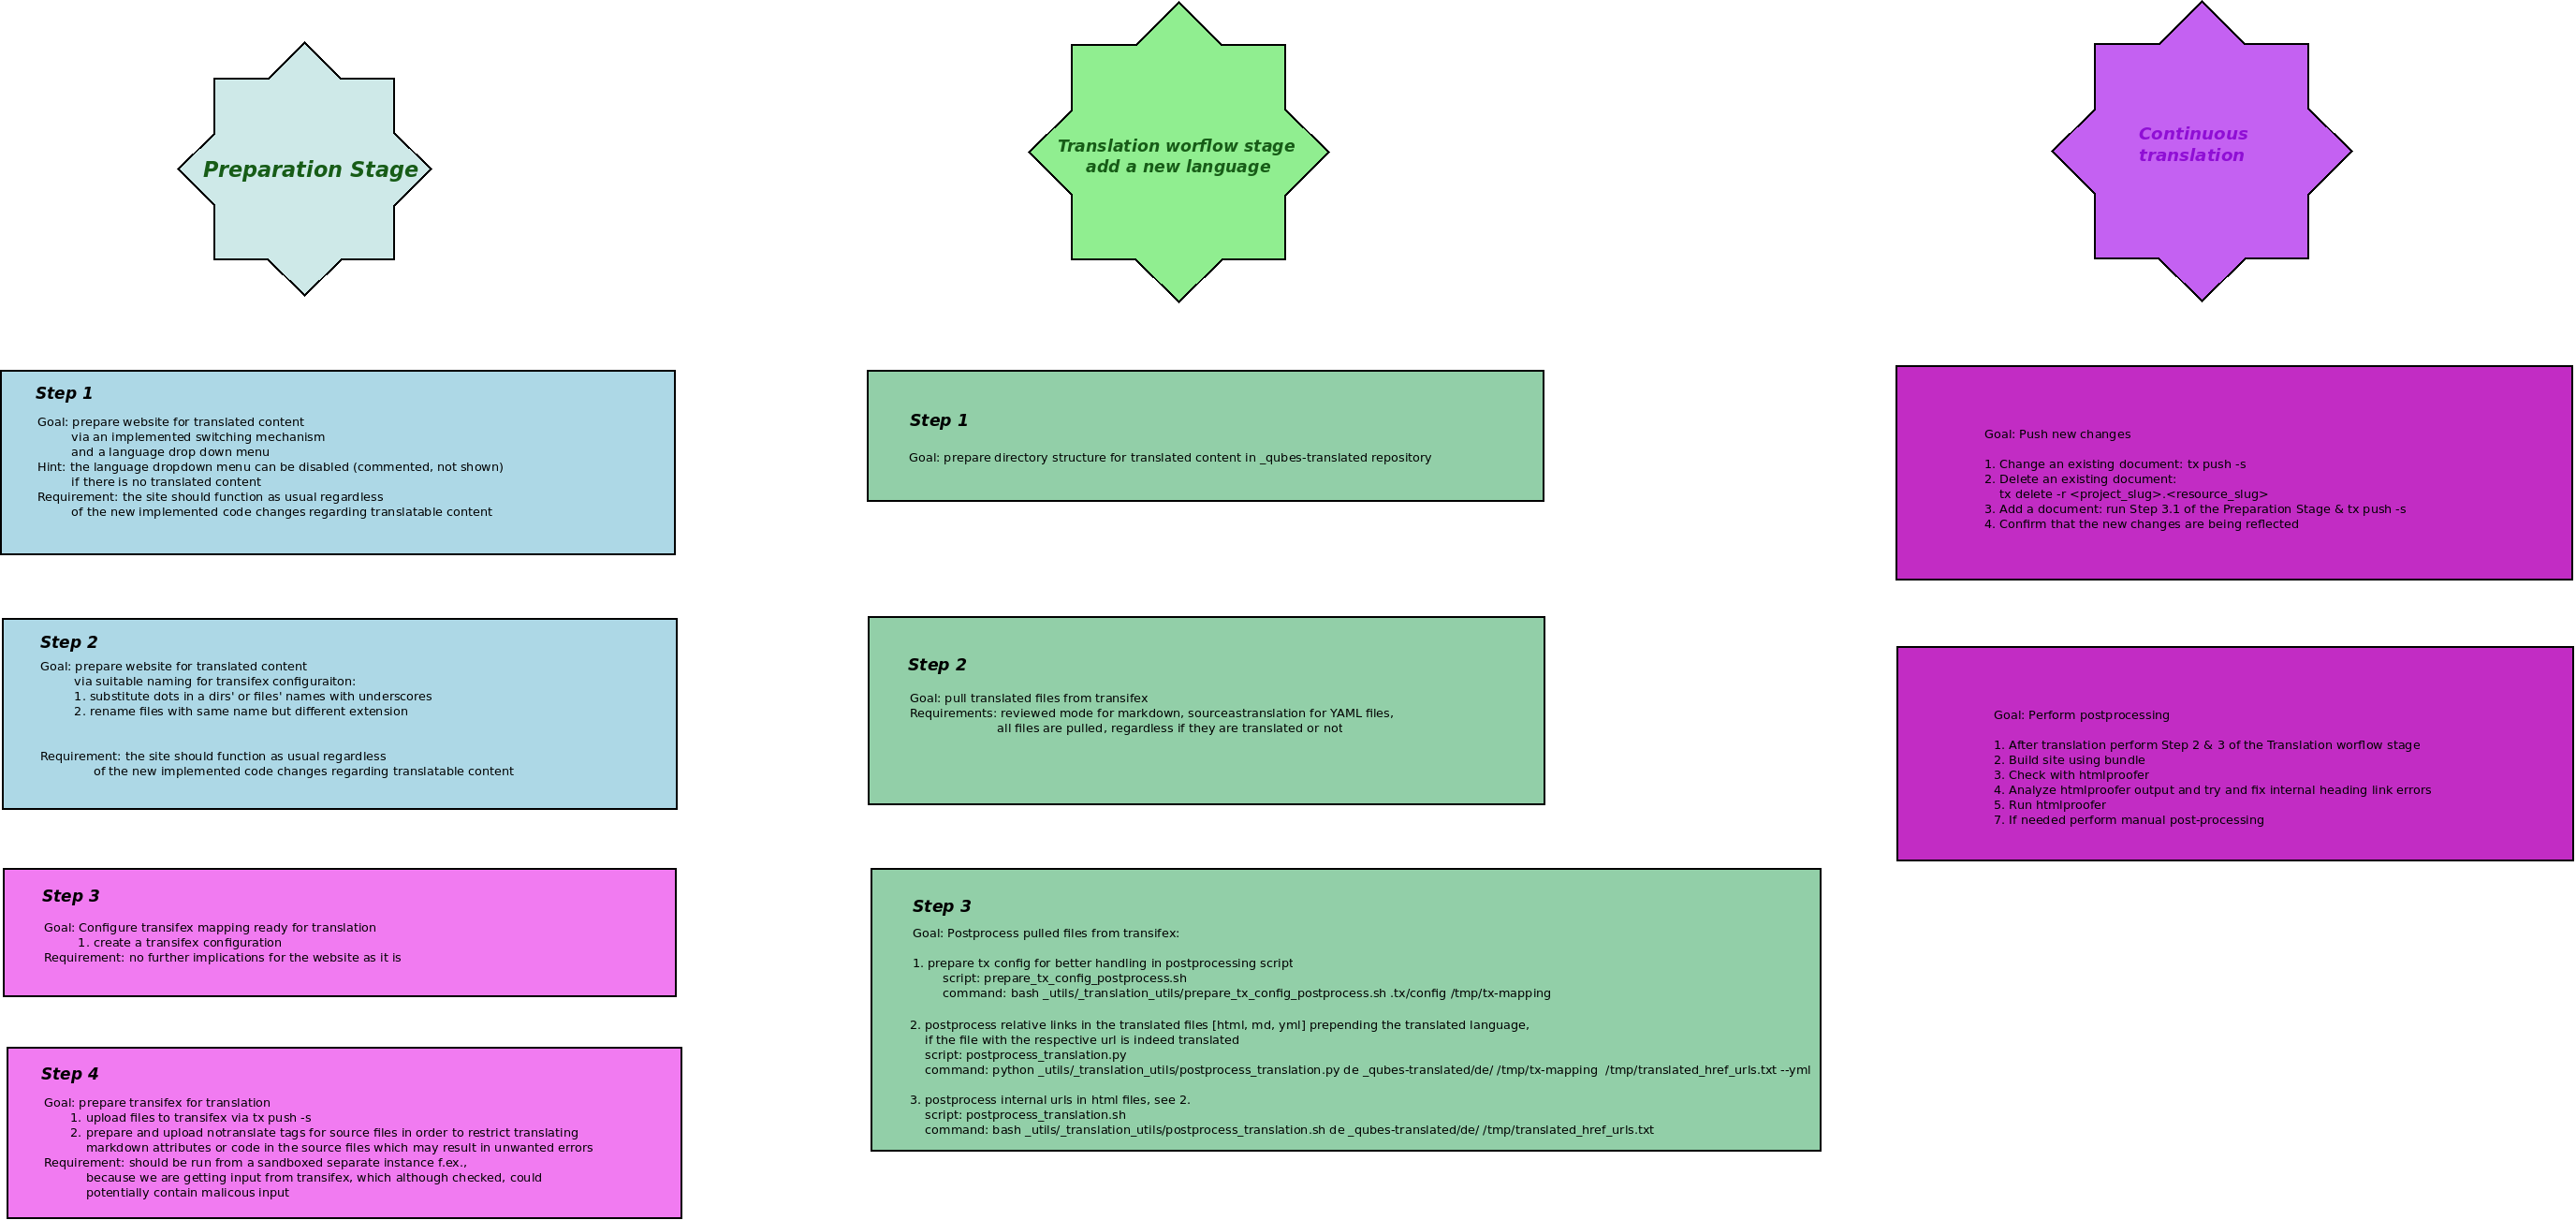
\includegraphics[width=\linewidth]{pix/mdworkflow.png}
		\caption{Localization of the official Qubes OS documentation workflow}
		\label{fig:mdworkflow}
	\end{figure}
\end{frame}



\begin{frame}
	\frametitle{Continuous localization of the official Qubes OS documentation (m)}
	\framesubtitle{As part of the official Qubes OS Website}
	\begin{itemize}
		\item TODO a pic m
	\end{itemize}	

\end{frame}


\begin{frame}
	\frametitle{Outlook for Markdown Qubes OS documentation (m)}
	\framesubtitle{As part of the official Qubes OS Website}
	
	\begin{itemize}
		\item Still a viable way forward
		\item Can be used for localization of the website
		\item TODOs:
		\begin{itemize}
			\item 
		\end{itemize}
	\end{itemize}


\end{frame}

\section{Where are we? The present}

\begin{frame}
	\frametitle{Read The Docs (m)}
	\begin{itemize}
		\item RTD - cons and pros
		\begin{itemize}
			\item versioned documentation
			\item supported translation
			\item transifex support
		\end{itemize}
		\item conversion 
		\begin{itemize}
			\item markdown to rst
			\item postprocessing rst files to fix broken links, cross-referencing
%			\item explain cross-referencing in sphinx 
		
		\end{itemize}
		\item transifex workflow
		\begin{itemize}
			\item transifex client shit
		\end{itemize}
		\item online RT documentation 
		\item new qubes-os website contents
		
		
	\end{itemize}
\end{frame}

\begin{frame}
	\frametitle{Continuous localization of the official Qubes OS documentation (m)}
	\framesubtitle{As RST on RTD}
	\begin{itemize}
		\item TODO a pic m
	\end{itemize}	
	
\end{frame}


\section{Quo vadis? The future}

\begin{frame}
	\frametitle{Looking forward (m)}
	\begin{itemize}
		\item official decision
		\item Testing and fixing bugs phase
		\item go live
		\item assign to translate with transifex walktrough
		\item official developer documentation already on RTD translation workflow proposal
		\item community documentation translation workflow proposal
		\item official website translation (pages, perhaps even posts)
	\end{itemize}
\end{frame}

\begin{frame}
	\frametitle{Specific tasks (1)(m)}
	\begin{itemize}
		\item Clean up the qubes os transifex project vocabularies
		\item Mark the uploaded files in Priority list as urgent
		\item Official translation Guidelines
		\item Translation FAQ
		\item Translation glossary
		\item Create github issue label translation
		\item Create translation issue template
		\item Create language specific documentation file inside the qubes-translation submodule for the specific language to be maintained by translators as a README.md Refer to it from the general language specific guidelines
		\item Update the general contribution guidelines
		\item Create a localization brief
		\item Create tutorial vids for translating/maintating
		
	\end{itemize}
\end{frame}

\begin{frame}
	\frametitle{Thank you!}
	\begin{center}
		Questions? Suggestions? 
	\end{center}
\end{frame}

\end{document}

